\documentclass[12pt, aspectratio=43]{beamer}
\usepackage[backend=bibtex, style=authoryear]{biblatex} % bibliography

% BEAMER TEMPLATE AND THEME
\setbeamertemplate{footline}[frame number]
\usetheme{Estonia}
\mode<presentation>
\AtBeginSection[]{
  \begin{frame}
  \vfill
  \centering
  \begin{beamercolorbox}[sep=8pt,center,shadow=true,rounded=true]{title}
    \usebeamerfont{title}\insertsectionhead\par%
  \end{beamercolorbox}
  \vfill
  \end{frame}
}

\addbibresource{../report/biblio.bib}

% TITLE PAGE
\title{Kubernetes cluster simulator based on Batsim}
\title{Development and evaluation of a Kubernetes cluster simulator based on
Batsim}

\author{\textbf{Presented by:} Théo Larue\\\textbf{Supervised by:} Olivier
Richard \& Michael Mercier}

\date{August 31, 2020}

\institute[Théo LARUE]{Université Grenoble Alpes}

\titlegraphic{
	\includegraphics[height=5ex]{../imgs/uga-logo.png}\hspace{2ex}
	\includegraphics[height=6ex]{../imgs/ENSIMAG.png}\hspace{2ex}
	\includegraphics[height=5ex]{../imgs/Logo-LIG.jpg}\hspace{2ex}
	\includegraphics[height=5ex]{../imgs/ryax-logo.png}
}

\begin{document}

\frame{\titlepage}

\begin{frame}\frametitle{Table of contents}\tableofcontents
\end{frame}

\section{Introduction}
\begin{frame}{Computer infrastructures}
	Distributed systems, many domains: Grid, Edge, HPC, Cloud, P2P, Volunteer, Cluster. 

	These systems are very complex. (some graph to illustrate the
	increase in size of supercomputers)
\end{frame}

\begin{frame}{Studying distributed systems}
	Why studying these infra? To test a system performances under varying
	loads, applications, scheduling policies, system size and topology. Or
	to develop new RJMS or research new scheduling algorithms.
\end{frame}

\begin{frame}{Studying distributed systems}
	How to study these infra? Too many elements and interactions to
	consider, so no theoretical study. 

	Real experiments are too costly (both in time and resources) and not
	reproducible.
\end{frame}

\begin{frame}{Studying distributed systems}
	Emulation resolves the issue of reproducibility.

	Simulation resolves both reproducibility and scalability
	issues.
\end{frame}

\section{Literature review}
\begin{frame}{Domain specific simulators}
	refs on domain specific simulators, summed up in a table. Explain
	briefly the concept behind some of them.
\end{frame}

\begin{frame}{Software specific simulators}
	YARNSim, SLURM simulator
\end{frame}

\begin{frame}{Publication specific simulators}
	``Publish and perish'' - Milian Poquet
\end{frame}

\begin{frame}{SimGrid}
	SimGrid: Versatile, scalable, accurate.

	Cpu = a computation speed.\\
	Storage = a seek time and a data transfert rate.\\
	Network = a flow model, modeling bandwith sharing behaviors of actual
	protocol.

	Simple models but thoroughly validated.
\end{frame}

\begin{frame}{Batsim}
	Aimed at studying RJMS.\\
	Strong decoupling decision process / simulator.
\end{frame}

\begin{frame}{Batsim - related work}
	Alea: modular, extensible.

	Accasim: supports additional information (temperature, power
	consuption). Very efficient in terms of simulation time and memory
	usage.

	Both outperform Batsim in terms of scalability. However it is not fair
	to compare them on this point because Batsim relies on well thought
	models, when these two only implement delay jobs.
\end{frame}

\begin{frame}{Kubernetes}
	Explain containers real quick.

	Container orchestration software, description based.
\end{frame}

\begin{frame}{Kubernetes cluster simulation}
	k8s-cluster-simulator: open source, student project, delay jobs.
	Schedulers provided via a Go interface.

	joySim: closed-source, fully fledged kubernetes cluster simulator,
	service oriented (mock nodes).
\end{frame}

\section{Integrating Kubernetes schedulers to Batsim}

\begin{frame}{Technical challenges}
	\begin{enumerate}
		\uncover<1->{\item Integration with Kubernetes.}
		\uncover<2->{\item Intercepting scheduler time.}
		\uncover<3->{\item Time synchronization between Batsim and the scheduler.}
	\end{enumerate}
\end{frame}

\begin{frame}{Batsim concepts}
	\begin{columns}
		\column{0.5\textwidth}
		\centering
		\includegraphics[width=\textwidth]{../imgs/batsim-sequence-diag.png}
		\tiny{source \url{https://batsim.readthedocs.io}}

		\column{0.5\textwidth}
		Batsim events and protocol.

		User defined workloads.

		(insert json examples?)
\end{columns}
\end{frame}

\begin{frame}{Kubernetes concepts}
	\centering
	\only<1>{\includegraphics[width=\textwidth]{../imgs/components-of-kubernetes.png}}
	\only<2>{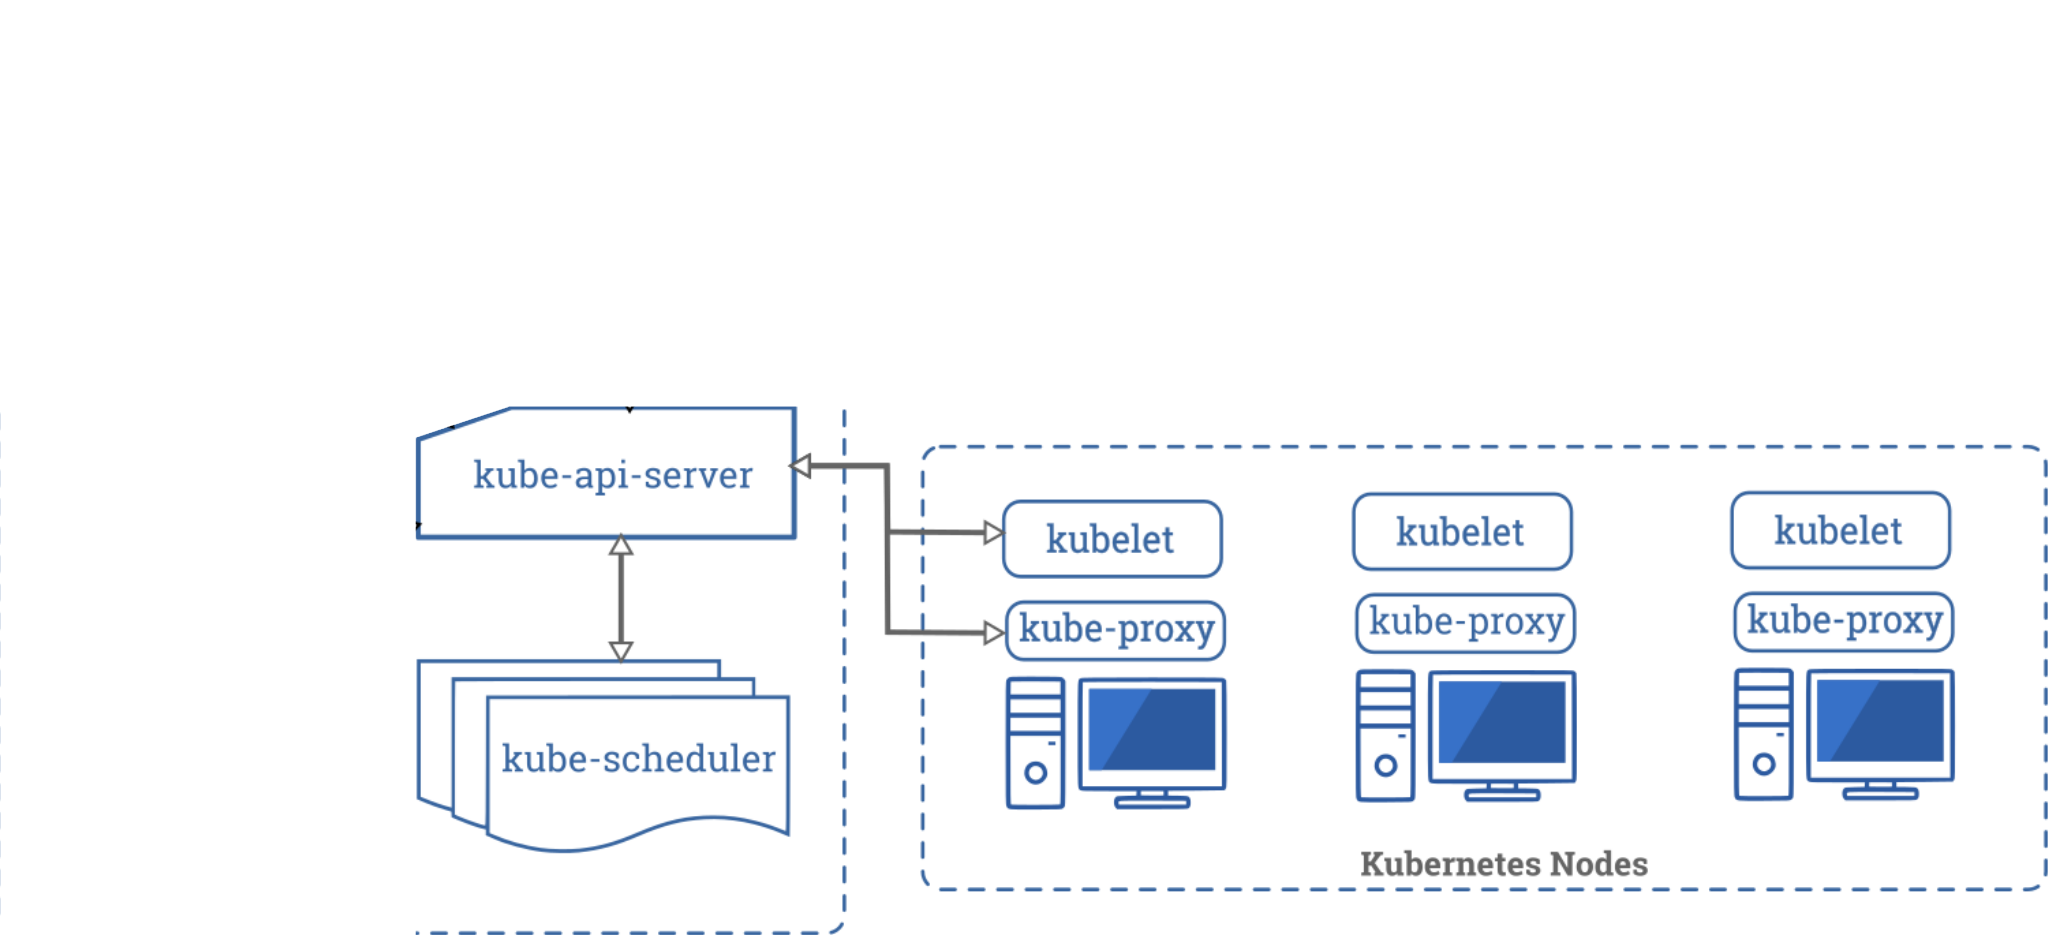
\includegraphics[width=\textwidth]{../imgs/components-of-kubernetes-2.png}}
	\tiny{source: \url{https://kubernetes.io/docs/concepts/overview/components/}}\\
	\small{Kubernetes components.}
\end{frame}

\begin{frame}{Batkube integration with Kubernetes}
	\centering
	\includegraphics[width=0.8\textwidth]{../imgs/custom-api.pdf}\\
	\small{Reimplementation of a custom API.}
\end{frame}

\begin{frame}{Architeture of Batkube}
	\centering
	\includegraphics[width=\textwidth]{../imgs/batkube-architecture-3-synchro.pdf}
	\small{Global architecture of Batkube.}
\end{frame}


\begin{frame}{Similar resources}
	\begin{columns}
		\column{0.5\textwidth}
		\centering
		\includegraphics[width=\textwidth]{../imgs/node-overview.png}
		\tiny{source: \url{https://kubernetes.io/docs/tutorials/kubernetes-basics/explore/explore-intro/}}

		\column{0.5\textwidth}
		\begin{block}{Translation between Kubernetes and Batsim}
			\begin{itemize}
				\item A Pod = a job.
				\item A Node = a compute resource.
			\end{itemize}
		\end{block}
	\end{columns}
\end{frame}


\begin{frame}{Time interception}
	\centering
	\includegraphics[width=0.6\textwidth]{../imgs/synchro-go-sources.pdf}\\
	\small{Schedulers are patched to redirect their time.}
\end{frame}

\begin{frame}{batsky-go}
	\begin{columns}
		\column{0.5\textwidth}
		\centering
		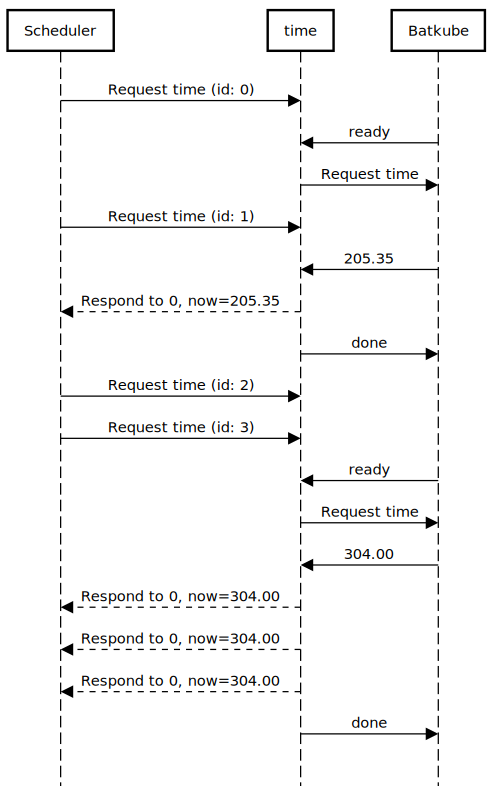
\includegraphics[scale=0.38]{../imgs/requester-broker.pdf}
		
		\column{0.5\textwidth}
		Exchanges between batsky-go (designed by ``time'') and Batsim
	\end{columns}
\end{frame}

\begin{frame}{Time synchronization}
	\centering
	\includegraphics[width=0.85\textwidth]{../imgs/lignes_de_temps.pdf}\\
	\small{Time synchronization between Batsim and the scheduler}
\end{frame}

\section{Study of the simulator}
\begin{frame}{Studied workloads and platforms}
\end{frame}

\begin{frame}{Minimum delay}
	TODO for future work: study min delay effect on makespan and mwt
\end{frame}

\begin{frame}{Timeout}
\end{frame}

\begin{frame}{Maximum simulation timestep}
	the max timestep onyl experiment did not how much. Need to couple it
	with a backoff multiplier experiment also.
\end{frame}

\begin{frame}{Experimentation on a real cluster}
	[ schema cluster emulé ]
\end{frame}

\begin{frame}{Deviation with reality}
	[meme table que dans le raport]
	Reprendre les analyses du rapport.
\end{frame}

\section{Discussion and future work}
\begin{frame}{Capabilities of Batkube}
	- delay jobs\\
	- cpu and memory requests\\
	- can patch any kubernetes scheduler written in Go\\
	- the api only supports the default scheduler
\end{frame}

\begin{frame}{Limitations}
	- memory hungry (in fact, the scheduler is memory hungry)\\
	- some problems with the scheduler\\
	- not scalable
\end{frame}

\begin{frame}{Perspectives for future work}
	- parallel jobs\\
	- storage\\
	- more complete api: support for more schedulers but also tools (monitoring tools)
\end{frame}

\begin{frame}[allowframebreaks]
        \frametitle{References}
	\printbibliography
\end{frame}

\end{document}

